\documentclass[10pt,a4paper,twocolumn,twoside]{article}
\usepackage[utf8]{inputenc}
\usepackage[catalan]{babel}
\usepackage{multicol}
\usepackage{graphicx}
\usepackage{fancyhdr}
\usepackage{times}
\usepackage{titlesec}
\usepackage{multirow}
\usepackage{svg}
\usepackage{booktabs}
\usepackage{tikz}
\usepackage{hyperref} 
\usepackage{caption}
\usepackage{lettrine}
\usepackage{lipsum}
\usepackage{cite}
\usepackage{amsmath}
\usepackage{amssymb}
\usepackage[top=2cm, bottom=1.5cm, left=2cm, right=2cm]{geometry}
\usepackage[figurename=Fig.]{caption}
%\captionsetup[table]{textfont=sc}
\setlength{\parskip}{1pt}
\titlespacing*{\section}{0pt}{*1.5}{*0.7}
\titlespacing*{\subsection}{0pt}{*1.2}{*0.5}
\setlength{\textfloatsep}{10pt plus 1pt minus 2pt}
\setlength{\floatsep}{8pt plus 1pt minus 1pt}
\setlength{\intextsep}{8pt plus 1pt minus 1pt}
\setlength{\abovedisplayskip}{6pt}
\setlength{\belowdisplayskip}{6pt}
\captionsetup[figure]{skip=10pt}
\captionsetup[table]{skip=6pt}
\titlespacing*{\section}{0pt}{12pt plus 3pt minus 1pt}{6pt plus 1pt minus 1pt}
\titlespacing*{\subsection}{0pt}{10pt plus 2pt minus 1pt}{5pt plus 1pt minus 1pt}
\titlespacing*{\subsubsection}{0pt}{4pt plus 1pt minus 1pt}{1pt plus 1pt minus 1pt}
\author{\LARGE\sffamily Pol Riubrogent Comas}
\title{\Huge{\sffamily From Dust to Detail: Deep Learning Pipelines for Analog Film Restoration}}
\date{}

\newcommand\blfootnote[1]{%
  \begingroup
  \renewcommand\thefootnote{}\footnote{#1}%
  \addtocounter{footnote}{-1}%
  \endgroup
}

%
%\large\bfseries\sffamily
\titleformat{\section}
{\sffamily\scshape\bfseries}
{\textbf{\thesection}}{1em}{}

\begin{document}

\fancyhead[LO]{\scriptsize POL RIUBROGENT COMAS: DEEP LEARNING
PIPELINES FOR ANALOG FILM RESTORATION}
\fancyhead[RO]{\thepage} \fancyhead[LE]{\thepage}
\fancyhead[RE]{\scriptsize EE/UAB TFG DADES: DEEP LEARNING
PIPELINES FOR ANALOG FILM RESTORATION}

\fancyfoot[CO,CE]{}

\fancypagestyle{primerapagina}
{
   \fancyhf{}
   \fancyhead[L]{\scriptsize TFG EN ENGINYERIA DADES, ESCOLA D'ENGINYERIA (EE), UNIVERSITAT AUTÒNOMA DE BARCELONA (UAB)}
   \fancyfoot[C]{\scriptsize June 2025, Escola d'Enginyeria (UAB)}
}

%\lhead{\thepage}
%\chead{}
%\rhead{\tiny EE/UAB TFG INFORMÀTICA: TÍTOL (ABREUJAT SI ÉS MOLT LLARG)}
%\lhead{ EE/UAB \thepage}
%\lfoot{}
%\cfoot{\tiny{February 2015, Escola d'Enginyeria (UAB)}}
%\rfoot{}
\renewcommand{\headrulewidth}{0pt}
\renewcommand{\footrulewidth}{0pt}
\pagestyle{fancy}

%\thispagestyle{myheadings}

\twocolumn[\begin{@twocolumnfalse}

%\vspace*{-1cm}{\scriptsize TFG EN ENGINYERIA DADES, ESCOLA D'ENGINYERIA (EE), UNIVERSITAT AUTÒNOMA DE BARCELONA (UAB)}
\renewcommand{\refname}{References}
\maketitle

\thispagestyle{primerapagina}
%\twocolumn[\begin{@twocolumnfalse}
%\maketitle
%\begin{abstract}
\begin{center}
\parbox{0.915\textwidth}
{\sffamily \small
%\end{abstract}
%\bigskip
%\begin{abstract}
\\
\textbf{Abstract--}Restoring analog film, such as 35mm prints, is traditionally a manual and time-consuming process, often limited to well-funded institutions. Recent deep learning methods offer a path to automation, but most fail to account for the unique visual characteristics of film, particularly its natural grain. This project explores two restoration approaches designed to selectively remove common physical defects like dust, scratches, dirt, and burned regions, while preserving the intrinsic texture of film scans. The first is a modular pipeline combining a damage segmentation network with an inpainting model; the second is an end-to-end transformer-based model adapted from Restormer. Both are trained on a synthetic dataset simulating real-world film degradation and are evaluated using SSIM, PSNR, LPIPS, and qualitative analysis. The full code as well as planification can be consulted in: \url{https://github.com/NIU1636486/TFG_FILM_RESTORATION}
\\
\\
\textbf{Keywords-- } Film restoration, analog cinema, deep learning, artifact segmentation, inpainting, transformers, film grain, digital restoration, computer vision\\
}

\bigskip

{\vrule depth 0pt height 0.5pt width 4cm\hspace{7.5pt}%
\raisebox{-3.5pt}{\fontfamily{pzd}\fontencoding{U}\fontseries{m}\fontshape{n}\fontsize{11}{12}\selectfont\char70}%
\hspace{7.5pt}\vrule depth 0pt height 0.5pt width 4cm\relax}

\end{center}

\bigskip

%\end{abstract}

{
\begin{center}
    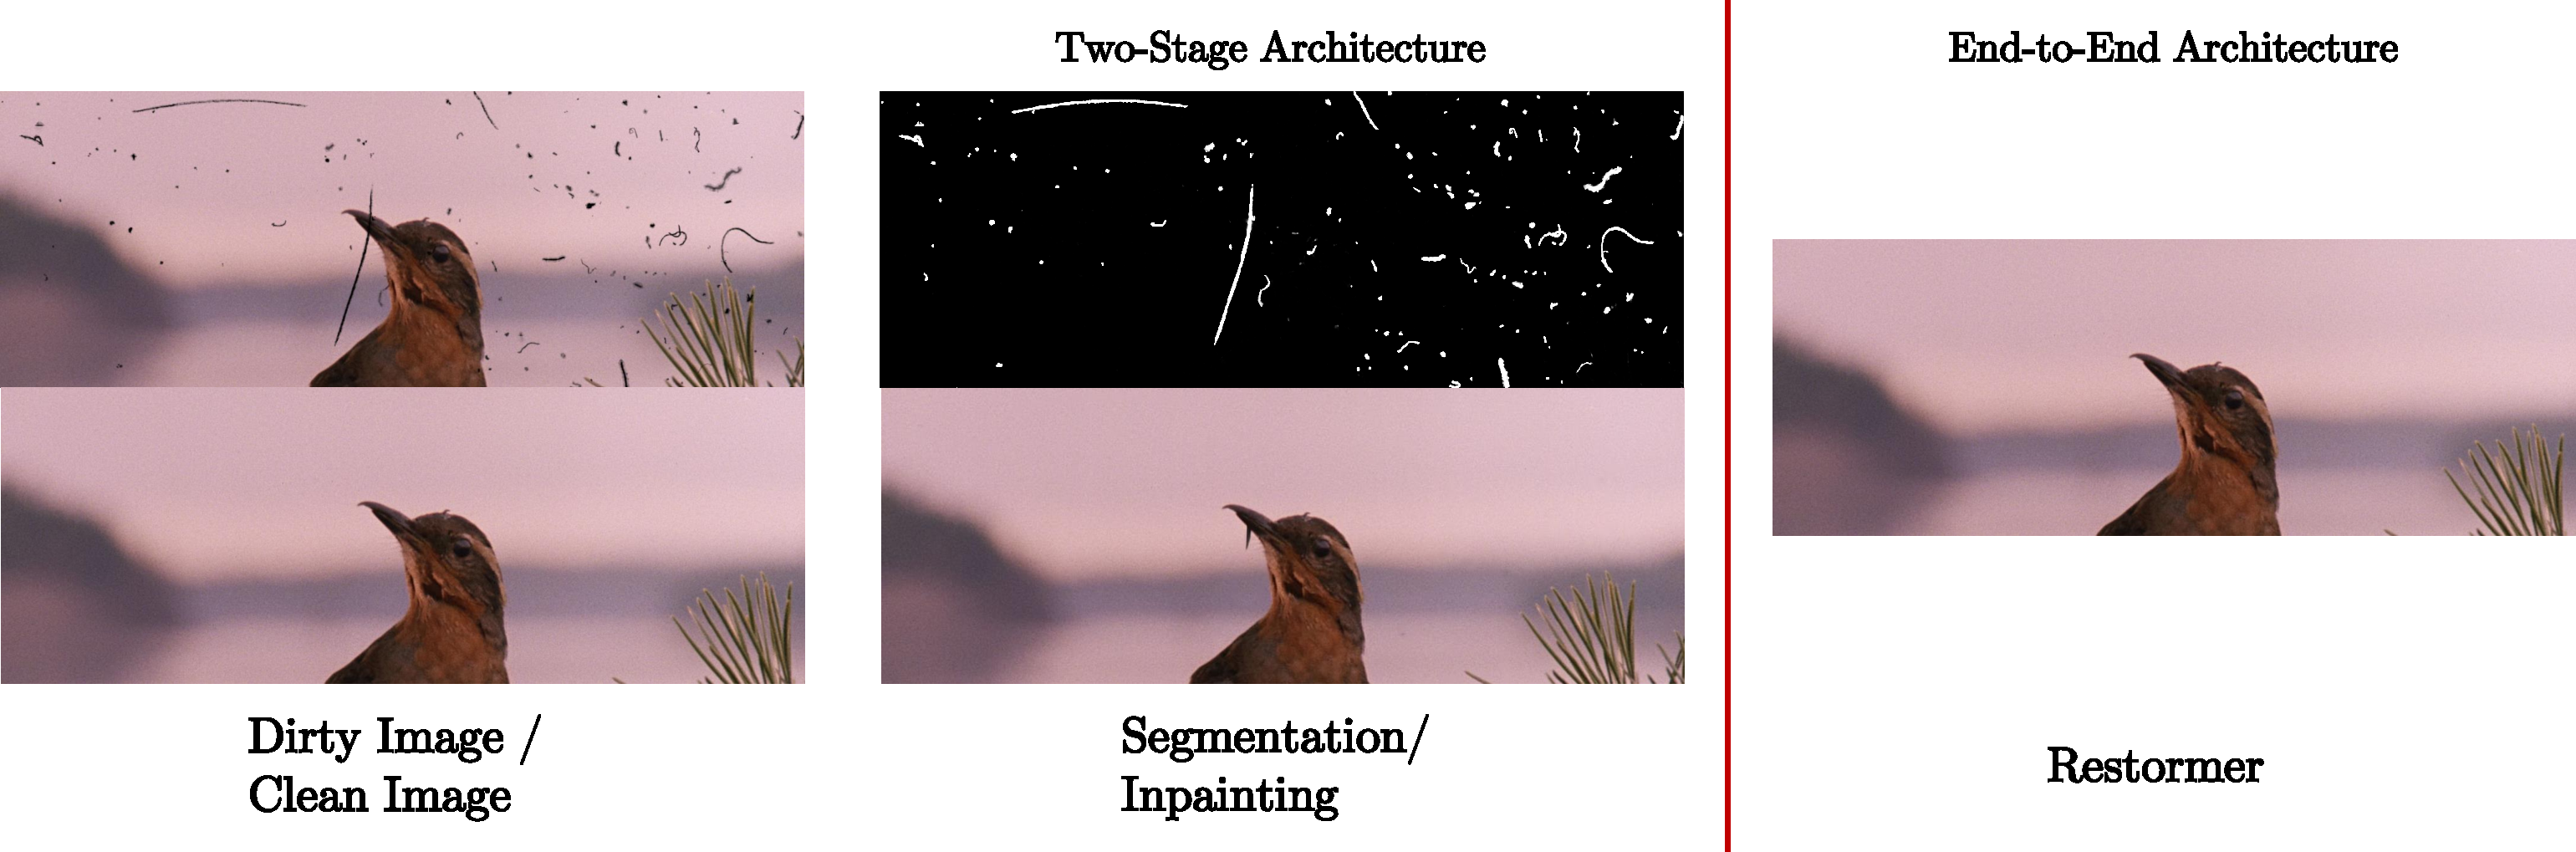
\includegraphics[width=\textwidth]{img/Portada.pdf}
    
    \captionsetup{type=figure}
    \captionof{figure}{Overview of the two restoration strategies: a two-stage pipeline with artifact segmentation and inpainting, and an end-to-end transformer model that restores degraded frames directly.}
    \label{fig:portada}
\end{center}
}

\blfootnote{$\bullet$ E-mail de contacte: pol.riubrogent@autonoma.cat}
\blfootnote{$\bullet$ Treball tutoritzat per: Ramon Baldrich Caselles (CVC, Color in Context)} \blfootnote{$\bullet$ Curs 2024/25}
\end{@twocolumnfalse}]


\section{Introduction}
\lettrine[lines=3]{T}{he} restoration of analog film footage, such as 35mm prints, remains a labor-intensive and time-consuming process. Traditional workflows rely on expert technicians manually cleaning reels or correcting scans frame by frame, often with the aid of rule-based software tools. While this yields curated results, especially when assisted by film specialists, it can take weeks or months to restore a single reel, rendering large-scale archival efforts prohibitively slow and expensive. As a result, restoration remains accessible primarily to well-funded institutions. The advent of deep learning has opened new possibilities to automate key steps in this process by learning to reconstruct damaged film regions while preserving historical and aesthetic fidelity. \\
Most deep learning approaches to image restoration have focused on generic tasks like denoising, super-resolution, or deraining (citation needed). Although architectures such as Restormer, LaMa, and DeepRemaster have demonstrated strong performance on these tasks, they are not tailored to the distinctive challenges of analog film degradation. In archival contexts, the objective is not merely to remove visible defects but to preserve the film’s intrinsic visual identity, most notably its characteristic grain. However, existing methods often smooth out this fine-grained structure, compromising perceptual fidelity. Moreover, there is limited exploration of the comparative effectiveness of different architectural paradigms, such as modular versus end-to-end designs. \\
This work proposes and evaluates two restoration strategies tailored to the specific demands of 35mm film scans. Unlike existing solutions that remove both noise and damage indiscriminately, the proposed methods explicitly preserve natural grain while removing acquired artifacts such as dust, scratches, hair, and burns. The first approach is a modular pipeline: a segmentation network locates damaged regions, which are then restored by a dedicated inpainting model. The second is an end-to-end transformer-based method based on Restormer, which performs restoration in a single pass. Both are trained on a synthetic dataset that simulates realistic film defects while retaining authentic grain. Evaluation is conducted using standard metrics, PSNR, SSIM, and LPIPS. \\
To address this challenge, the remainder of the work is organized as follows. First, I examine relevant prior efforts in image restoration, situating this project within the broader landscape of deep learning techniques. I then describe the construction of a domain-specific synthetic dataset tailored to film restoration. Next, two architectural strategies are detailed: a modular pipeline that separates defect detection and correction, and a transformer-based end-to-end model. Each is evaluated using both objective metrics and perceptual criteria. Finally, I discuss the comparative performance of these approaches, reflect on their limitations, and suggest directions for future research.

\section{Related Work}
Before the advent of digital tools, analog film restoration was an entirely manual endeavor. Archivists physically cleaned and reconditioned film reels to remove dust, mold, and dirt, often using specialized solvents and lint-free wipes. Torn or decayed frames were painstakingly repaired by splicing breaks with tape or glue, and severely damaged sequences could be salvaged by optical printing – re-photographing each frame to produce a new copy that bypasses scratches or warped sections. With the transition to scanned film, classical digital techniques emerged to accelerate restoration. Early software systems deployed rule-based defect detectors and morphological filters to identify artifacts like dust specks and vertical scratches, followed by image inpainting or interpolation to fill in those regions. While these hand-crafted pipelines improved consistency over purely manual repair, they often required expert tuning and struggled with complex degradations, setting the stage for data-driven restoration approaches in subsequent work. \cite{croci2015advanced}

\subsection{Restoration of Analog Film Scans}
Restoring analog film scans poses unique challenges due to the need to remove defects like dust, scratches, and dirt without erasing the fine-grained texture that defines their aesthetic. Existing methods, ranging from GAN-based inpainting \cite{gan} to CNNs optimized for PSNR and SSIM, often yield visually clean results but treat film grain as noise, leading to overly smoothed outputs that undermine archival fidelity. Furthermore, few works systematically compare architectural paradigms, leaving open questions about the relative merits of modular versus end-to-end approaches. \cite{survey} \\ 
\subsection{Modular Restoration: Segmentation Followed by Inpainting}
The FILM-AA framework exemplifies a modular strategy, employing a two-stage pipeline: a segmentation network trained on high-resolution labeled scans identifies damaged regions, and an inpainting model restores only those areas. This approach emphasizes interpretability and minimal intervention, key values in heritage restoration, by preserving untouched content and offering fine control. However, it does not explore architectural variants or assess the integration of advanced generative models, limiting its adaptability and generalizability.\\
\subsection{Transformer-Based Approaches for Image Restoration: Restormer}
In contrast, transformer-based vision models have recently achieved state-of-the-art results in generic restoration tasks such as denoising, deblurring, and super-resolution. Restormer is a leading example, designed for high-resolution image restoration through a hierarchical encoder-decoder architecture with multi-scale skip connections. Its ability to model both global structure and fine-grained texture makes it a promising candidate for analog film restoration. \\
Unlike modular approaches, Restormer operates end-to-end, implicitly learning to localize and correct degradations without auxiliary supervision. This implicit design offers flexibility but risks removing authentic features such as film grain if the learned prior becomes overly aggressive. \\
Restormer follows the principles of Vision Transformers (ViTs)~\cite{dosovitskiy2020image}, processing images via patch embeddings and multi-head self-attention across transformer layers. Unlike ViTs for classification, which collapse spatial information, Restormer retains resolution throughout, making it well-suited for dense restoration tasks.


\section{Dataset}
\label{sec:dataset}
A critical component of this project is the construction of a dataset suitable for training and validating a model capable of identifying and restoring visual artifacts in digitalized film footage, while preserving the inherent characteristics of celluloid film such as its grain structure. Unlike many existing image restoration datasets, such as LSDIR, which are primarily focused on tasks like super-resolution and general noise removal, the current objective demands a domain-specific dataset centered on real-world film degradation. These degradations include dust, dirt, hairs, and/or scratches, which are not unique to analog film but are also integral to the authenticity of the viewing experience. \\
Due to the lack of publicly available, large-scale datasets tailored to this specific restoration task, a synthetic dataset has been created as the primary training resource. This dataset construction process was designed to ensure both the visual realism and structural diversity necessary to support the development and evaluation of the two distinct restoration architectures proposed in this work. As will be explained in later sections, these architectures require differently structured data splits and target outputs, even though they share a common generation pipeline. In this section, two datasets will be introduced: a synthetic dataset created specifically for this task and the Documartica dataset, an externally provided dataset created similarly, but with unrelated images. Example images of each dataset can be seen in Appendix A.
\subsection{Synthetic Dataset}
The core dataset comprises high-resolution film frames artificially degraded with pixel-accurate artifact masks. Clean frames were extracted from a curated set of uncompressed Blu-ray restorations of 35mm films from the 1960s–1980s, selected for their faithful analog texture and visible grain. \\ To encourage generalization, the dataset was split using a stratified, non-random strategy: the test set includes full films and styles (e.g., animation) excluded from training. This ensures performance is evaluated not only on unseen frames but also on novel content and aesthetic domains.
\subsubsection{Artifact generation}
For artifact synthesis, this work employs the FILM-AA framework \cite{ivanova23analogue}, a publicly available library that provides extremely high-resolution 4K scans of damaged archival film, labeled pixel by pixel for each type of artifact. These scans and labels are then used to generate over 6000 different masks simulating film degradation. This on-the-fly composition strategy introduces diversity into the training set while maintaining precise control over ground truth artifact locations, which is crucial for supervised segmentation. In Fig. \ref{fig:artifacts} the different artifact types generated by this method can be seen. \\
\begin{figure}[h!]
    \centering
    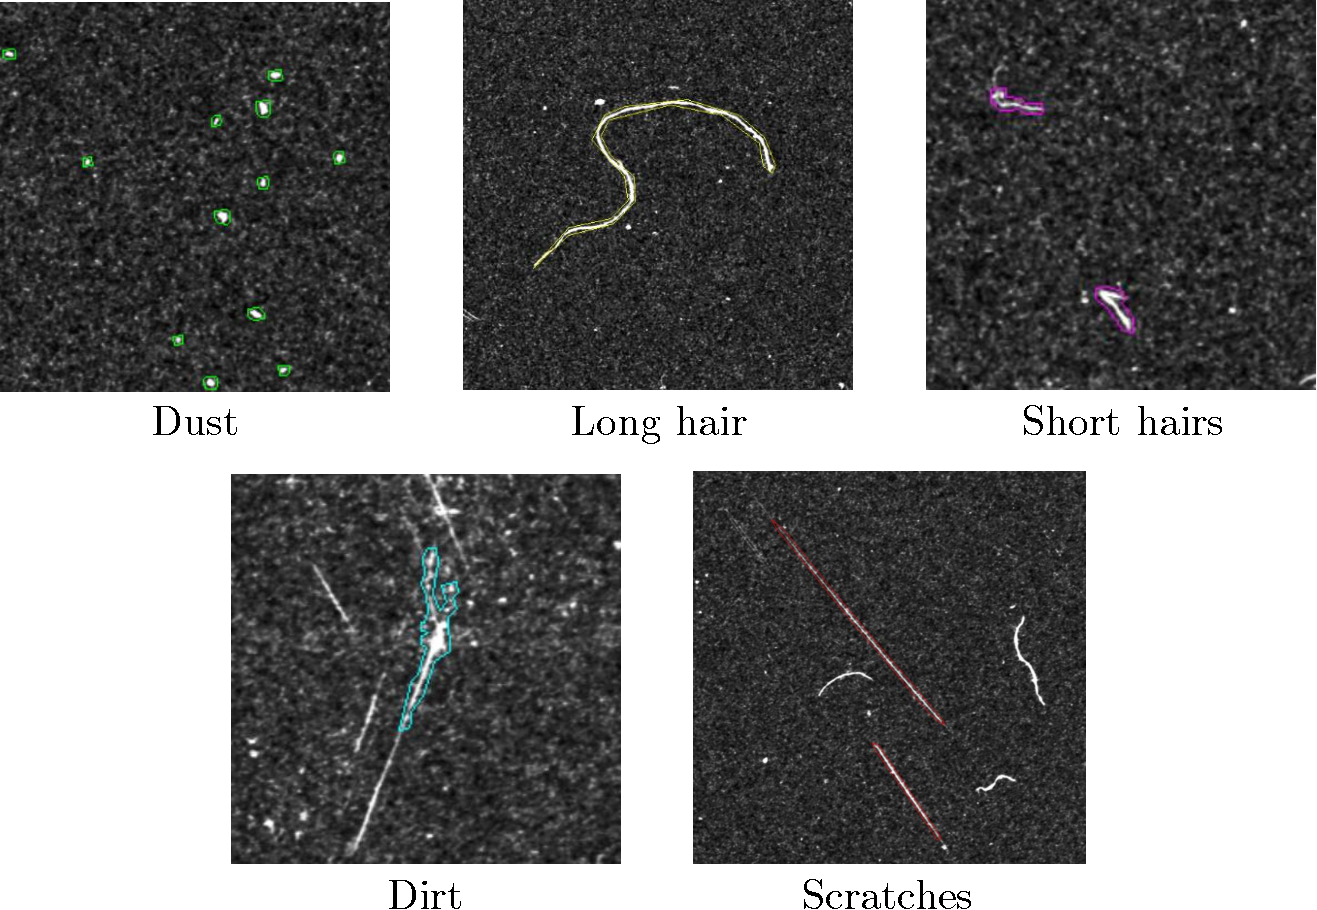
\includegraphics[width=\linewidth]{img/Artifacts.pdf}
    \caption{ \small Example damage artifacts for each type, including a section from one of the high-resolution scans used as a source for the damage.}
    \label{fig:artifacts}
    \vspace{-1em}
\end{figure}
\begin{figure*}[t]
  \centering
    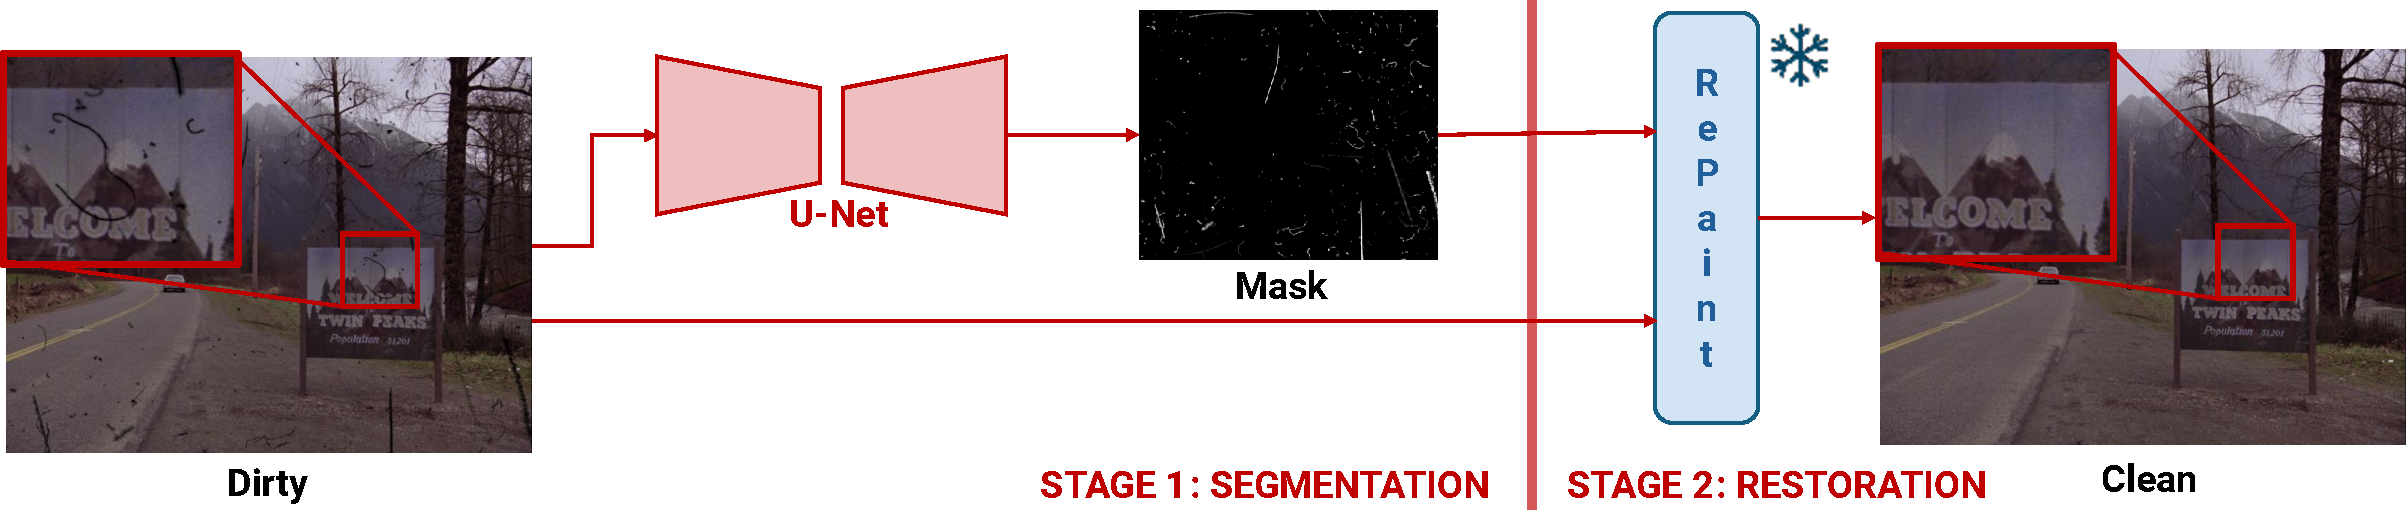
\includegraphics[width= \textwidth]{img/Diagrama_Two_Stage_BO.pdf}\vspace{-0.6em}
    \caption{ \small
Overview of the proposed two-stage restoration architecture. A U-Net-based model first segments visual artifacts (e.g., dust, dirt, scratches) from a degraded film frame into a binary mask; both the frame and mask are then input to RePaint~\cite{repaint}, a pretrained diffusion-based inpainting model.
}
    \label{fig:two-stage}
\end{figure*}

To improve the visual realism of the composite images and reduce overfitting to sharp, high-contrast edges, the artifact masks were post-processed by applying a Gaussian blur around their borders. This blurring simulates the more natural and diffuse integration of artifacts into real film material and encourages the model to lean towards broader contextual features.
\subsection{Documartica Dataset}
In addition to the primary synthetic dataset, this work leverages a secondary dataset for pretraining purposes. Proved through direct contact from the authors of the FILM-AA paper, this dataset was generated using the same artifact simulation methodology described above, but was applied to a different base: high-resolution scans of 35mm still film frames from various, unspecified sources. \\ Although the Documartica dataset does not directly match the final application domain of degraded motion picture footage, it shares many visual features that are relevant for learning transferable representations.
\section{Two-Stage Arquitecture}
This work adopts a modular architecture for film restoration, explicitly separating defect localization and image reconstruction into two sequential stages. The first stage employs a segmentation network to identify damaged regions in the input frame by generating a binary mask, while the second stage uses a generative inpainting model to selectively restore only the corrupted areas, leaving intact regions unaltered. This design emulates traditional restoration workflows and provides enhanced control, minimizing the risk of unnecessary modifications and preserving subtle features such as film grain. A schematic overview is shown in Fig.~\ref{fig:two-stage}. The remainder of this section focuses on the segmentation component, as the inpainting stage (based on RePaint) is used without modification. \\
This modular separation also offers important methodological benefits. By decoupling damage detection from content generation, it allows for independent supervision of the segmentation task, increasing transparency and interpretability in what the model chooses to modify. Additionally, it facilitates the integration of domain-agnostic, state-of-the-art generative models, such as RePaint, without requiring end-to-end retraining, thereby enhancing flexibility and extensibility. In contrast to end-to-end architectures that regress directly from corrupted to restored frames, this design aligns more closely with archival restoration principles: intervene only when necessary and preserve the original wherever possible.
\subsection{Stage 1: Artifact Segmentation}
The segmentation network is responsible for detecting and localizing visual artifacts such as dust, dirt, hair, and scratches in film frames. This is formulated as a pixel-wise binary classification problem, where each pixel is labeled as either damaged or clean. The segmentation stage outputs a binary mask $M \in \{0,1\}^{H\times M}$ corresponding to an input image $I \in \mathbb{R}^{H\times M \times 3}$, where a value of 1 indicates the presence of a defect.\\ Given the requirements of precise spatial location and robustness to small-scale features, this work explores three variations of the U-Net architecture: \textbf{vanilla U-Net} \cite{unet}, \textbf{Attention U-Net} \cite{attunet}, and \textbf{R2AttUNet} \cite{r2attunet}. All three models share the characteristic encoder-decoder structure of U-Net, with skip connections linking encoder and decoder layers at corresponding scales to preserve spatial detail.
\subsubsection*{U-Net}
The original U-Net architecture \cite{unet} was designed for biomedical image segmentation, but has demonstrated strong performance on tasks requiring high-resolution spatial predictions. Its key strength lies in the ability to recover fine detail through its symmetric structure and skip connections, which is essential in the current task, where defects can span only a few pixels.
\subsubsection*{Attention U-Net}
To enhance the network's focus on relevant regions, Attention U-Net \cite{attunet} integrates attention gates into the skip connections, allowing the model to learn where to concentrate its representational capacity. This is particularly useful in this task, where the artifacts of interest, such as faint scratches, may otherwise be drowned out by dominant background structures or noise. The attention mechanism improves recall of small and subtle features while suppressing irrelevant activations.
\subsubsection*{R2AttUnet}
The Recurrent Residual Attention U-Net~\cite{r2attunet} extends previous architectures by integrating residual and recurrent connections into both encoder and decoder paths. Recurrent convolutions iteratively refine features, enabling the model to capture temporal dependencies even from single frames, while residual links stabilize training and support deeper representations. This design is particularly effective for restoring faint or textured artifacts that require broader contextual reasoning across spatial scales.
\subsubsection{Training Objective}
All models are trained using a standard Binary Cross Entropy (BCE) \cite{bceloss }loss function:
\begin{equation*}
    \mathcal{L}_{BCE} = -\frac{1}{N} \sum^N_{i=1}[y_ilog(\hat{y}_i)+(1-y_i)log(1-\hat{y}_i)]
\end{equation*}
where $\hat{y_i} \in [0,1]$ is the predicted probability for pixel $i$ and $y_i\in\{0,1\}$ is the corresponding ground truth label. The BCE loss penalizes false positives and false negatives symmetrically, making it suitable for binary segmentation tasks where class imbalance may be significant.
\subsection{Stage 2: Mask-Guided Inpainting}
\begin{table*}
\begin{center}
\caption{\small \underline{\textbf{Segmentation}} on Seen and Unseen evaluation splits for U-Net variants trained without pretraining and with pretraining. Unseen data comprises films and styles excluded from training, testing generalization to novel domains. Consistently, the best-performing model is the Pretrained U-Net using the Documartica dataset.}
\label{table:seg_only}
\vspace{-2mm}
\setlength{\tabcolsep}{8pt}
\scalebox{0.75}{
\begin{tabular}{l 
c c | c c || 
c c | c c c}
\toprule[0.15em]
\textbf{Method} 
& \multicolumn{4}{c||}{\textbf{Segmentation}} 
& \multicolumn{5}{c}{\textbf{Average}} \\
\cmidrule(lr){2-5} \cmidrule(lr){6-10}
& IOU $\uparrow$& DICE $\uparrow$ & IOU $\uparrow$ & DICE $\uparrow$ 
& IOU $\uparrow$& DICE$\uparrow$ & PSNR$\uparrow$ & SSIM$\uparrow$ & LPIPS$\downarrow$ \\
& \multicolumn{2}{c|}{Seen} & \multicolumn{2}{c||}{Not Seen}
& \multicolumn{2}{c|}{Segmentation} & \multicolumn{3}{c}{Inpainting} \\
\midrule[0.15em]
Base U-Net              & \underline{0.8628} & 0.9237 & \underline{0.8315} & \underline{0.9056}  & \underline{0.8472} & \underline{0.9147} & 24.59 & \underline{0.9758} & 0.0411 \\
Base AttU-Net           & 0.8606 & 0.9231 & 0.8264 & 0.9021  & 0.8435 & 0.9126 & 24.52 & \underline{0.9758} & 0.0412 \\
Base R2AttU-Net         & 0.7029 & 0.8234 & 0.7008 & 0.8218  & 0.7018 & 0.8226 & 16.70 & 0.9646 & 0.1692 \\
\midrule
Pretrained U-Net        & \textbf{0.8666} & \textbf{0.9271} & \textbf{0.8419} & \textbf{0.9122}  & \textbf{0.8542} & \textbf{0.9197} &   \underline{25.5895}    &   \textbf{0.9758}    &   0.0400    \\
Pretrained AttU-Net     & 0.8622 & \underline{0.9245} & 0.8291 & 0.9045  & 0.8457 & 0.9145 &   \textbf{26.0835}   &   0.9757    &   \underline{0.0395}    \\
Pretrained R2AttU-Net   & 0.6490 & 0.7860 & 0.6501 & 0.7868  & 0.6496 & 0.7864 &   17.0575    &   0.9563    &   0.2278    \\
\midrule
Denoising Pretrained U-Net    & 0.8019 & 0.8894 & 0.8004 & 0.8884  & 0.8012 & 0.8889 &   25.7950    &   0.9755    &   \textbf{0.0387  }  \\
Denoising Pretrained AttU-Net & 0.7923 & 0.8833 & 0.7904 & 0.8821  & 0.7914 & 0.8827 &   25.7121    &   0.9746    &   0.0409    \\
\bottomrule[0.1em]
\end{tabular}}
\end{center}
\vspace{-1.5em}
\end{table*}




Once an artifact mask is predicted, it is passed, along with the original degraded image, to an inpainting model that restores only the masked regions. This selective restoration is performed using \textbf{RePaint} \cite{repaint}, a state-of-the-art method based on Denoising Diffusion Probabilistic Model (DDPMs) \cite{ddpm}. RePaint is particularly well-suited to this problem due to its ability to handle arbitrary and irregular masks without task-specific training.\\
RePaint operates by conditioning a pre-trained, unconditional diffusion model during the reverse diffusion process. At each denoising step, the known (unmasked) pixels are reinjected into the diffusion trajectory, effectively guiding the model to preserve the surrounding context. The algorithm alternates between forward (re-noising) and backward (denoising) diffusing steps, a resampling strategy designed to iteratively harmonize the generated content with the original image structure. This mechanism ensures that the inpainted regions blend seamlessly into the surrounding context, an essential process for inpainting tasks, where the more telling section in inpainting is the seams of the inpainted regions.
\subsection{Experimental Setup}

To rigorously evaluate the proposed two-stage restoration pipeline, a series of experiments were conducted involving both segmentation and inpainting components. The segmentation models were tested under multiple architectural variants and pretraining configurations, while the inpainting stage employed a pretrained generative diffusion model in a mask-guided setup.

\subsubsection{Segmentation Model Training}

The segmentation task is formulated as binary pixel-wise classification, where the objective is to detect and localize visual artifacts, such as dust, dirt, hair, and scratches, in synthetic film frames. Three variants of the U-Net architecture were evaluated: the standard U-Net~\cite{unet}, the Attention U-Net~\cite{attunet}, and R2AttUNet~\cite{r2attunet}.

Each model receives a clean film frame and a synthetic artifact mask used to generate a degraded frame. While artifact masks are assigned randomly across the dataset, this randomness is seeded during training to ensure comparability across experiments. This deterministic sampling is later relaxed during testing to evaluate robustness under variability.

All models are trained for 60 epochs with a batch size of 4 and a learning rate of $4 \times 10^{-3}$. The optimization objective is the Binary Cross Entropy (BCE) loss:

\begin{equation*}
\mathcal{L}_{BCE} = -\frac{1}{N} \sum_{i=1}^{N} \left[ y_i \log(\hat{y}_i) + (1 - y_i) \log(1 - \hat{y}_i) \right]
\end{equation*}

\subsubsection{Pretraining Strategies}

To assess the impact of initialization on segmentation performance, four pretraining strategies were explored:

\begin{itemize}
    \item \textbf{No pretraining}: Random weight initialization.
    \item \textbf{Denoising pretraining}: Following Brempong et al.~\cite{denoise}, a denoising task was used to initialize weights. The model was trained for 10 epochs to reconstruct clean images from synthetic Gaussian noise ($\mu=0$, $\sigma=25/255$), a setting commonly used in pretext tasks.
    \item \textbf{Domain-specific pretraining}: Initialization via training on the Documartica dataset using the same artifact synthesis pipeline.
\end{itemize}

These experiments aim to determine whether task-aligned or domain-aligned representations yield stronger generalization on the segmentation task.

\subsubsection{Segmentation Evaluation Metrics}

Segmentation performance is assessed using the Dice coefficient (DSC) and Intersection-over-Union (IoU)~\cite{segmetrics}:

\begin{align*}
    \text{DSC} &= \frac{2 |Y \cap \hat{Y}|}{|Y| + |\hat{Y}|} \\
    \text{IoU} &= \frac{|Y \cap \hat{Y}|}{|Y \cup \hat{Y}|}
\end{align*}

Here, $Y$ and $\hat{Y}$ denote the ground truth and predicted binary masks, respectively. Both metrics are computed at the pixel level over a held-out validation set. The Dice coefficient is particularly sensitive to class imbalance, which is critical in this task as the majority of pixels in each frame are undamaged. IoU penalizes false positives and false negatives more strictly and is especially useful for quantifying over-segmentation, which may lead to excessive inpainting and visual overcorrection.

\subsubsection{Inpainting with RePaint}

The second stage of the pipeline restores corrupted regions using RePaint~\cite{repaint}, a diffusion-based inpainting model. RePaint operates on 256$\times$256 inputs and was used without retraining. Due to this resolution constraint, a patch-wise inference strategy is adopted: each input frame is divided into overlapping 256$\times$256 patches, which are inpainted independently and then stitched together to reconstruct the full-resolution frame.

Although this limits the model’s access to global context, it offers a practical solution under computational constraints. Training a custom diffusion model was considered infeasible given the timeframe of this project.
\subsubsection{Restoration Evaluation Metrics}
\label{experimental_setup_metrics}
To evaluate the overall restoration quality of the two-stage system, three widely used image quality metrics were employed: PSNR, SSIM \cite{psnrssim}, and LPIPS.
Both PSNR and SSIM are calculated straightforwardly with the following formulas:
\begin{align*}
    \text{PSNR}(y,\hat{y}) =& \;10\;log_{10} \left( \frac{255^2}{MSE(y,\hat{y})}\right)\\
   \text{SSIM}(y, \hat{y}) =& \;\frac{(2\mu_y\mu_{\hat{y}} + C_1)(2\sigma_{y\hat{y}} + C_2)}{(\mu_y^2 + \mu_{\hat{y}}^2 + C_1)(\sigma_y^2 + \sigma_{\hat{y}}^2 + C_2)}
\end{align*}
where $\mu_y$ and $\mu_{\hat{y}}$ are the means of $y$ and $\hat{y}$, $\sigma_y^2$ and $\sigma_{\hat{y}}^2$ are their variances, $\sigma_{y\hat{y}}$ is the covariance between $y$ and $\hat{y}$, and $C_1$, $C_2$ are constants to stabilize the division. \\
LPIPS (Learned Perceptual Image Patch Similarity)\cite{lpips} quantifies perceptual similarity by comparing deep feature activations from pretrained networks, specifically AlexNet\cite{alexnet} in this work. Unlike pixel-wise metrics, LPIPS better reflects human visual perception and is particularly effective at capturing subtle differences in texture and structure, making it well-suited for evaluating the fidelity of restored regions. \\ To assess both accuracy and non-invasiveness, metrics were computed globally (entire image) and locally (inpainted regions only), ensuring that restorations corrected defects while preserving undamaged content.

\subsection{Results and Discussion}
This section reports the quantitative and qualitative outcomes of the proposed two-stage restoration pipeline, analyzing how segmentation model architecture and pretraining strategies influence final restoration quality. Evaluation is conducted over two validation splits: Seen, which contains previously unexposed frames from films included in the training set, and Unseen, composed of entirely different films and aesthetic domains excluded from training. This design tests both generalization within-domain and robustness to stylistic shifts.

\subsubsection{Segmentation Performance}
Among the models trained from scratch, both the vanilla U-Net and Attention U-Net achieve consistently strong results across both evaluation subsets. On average, they reach Dice coefficients above 0.90 and IoU values exceeding 0.84. These segmentation masks translate into high-quality inpainting outputs, with LPIPS around 0.04 and SSIM surpassing 0.97, indicating that the mask quality is sufficient to guide precise artifact removal. In contrast, the R2AttUNet architecture, despite its increased complexity through recurrent and residual pathways, performs significantly worse across all segmentation metrics. It yields notably lower Dice and IoU scores, with LPIPS nearly four times higher than its counterparts and a PSNR reduction exceeding 7 dB. Given this consistent underperformance, R2AttUNet is excluded from subsequent experiments. 
\begin{figure}[htbp]
    \centering
    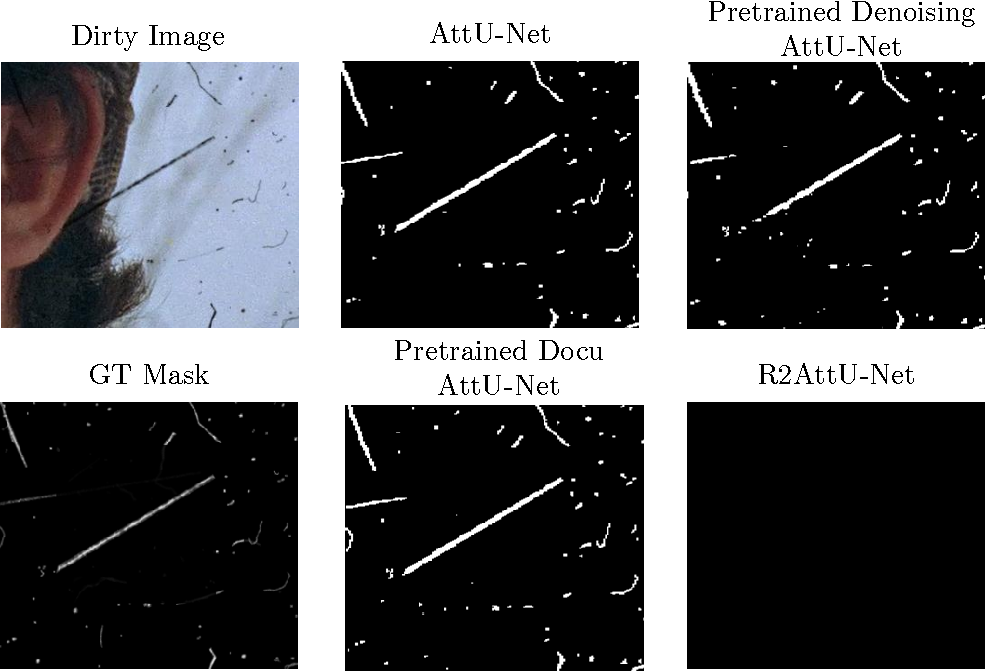
\includegraphics[width=0.8\linewidth]{img/segmentation_figure.pdf}
    \caption{\small Comparison of three of the AttU-Net experiments, along twith he baseline R2AttU-Net. It can be observed that all of the AttU-Net perform equally, varying just in the contours of artefacts. The R2AttU-Net does not perform as expected. This is hypothesized that this is due to undertraining the model.}
    \label{fig:segmentation_performance}
\end{figure}
\begin{figure}[htbp]
    \centering
    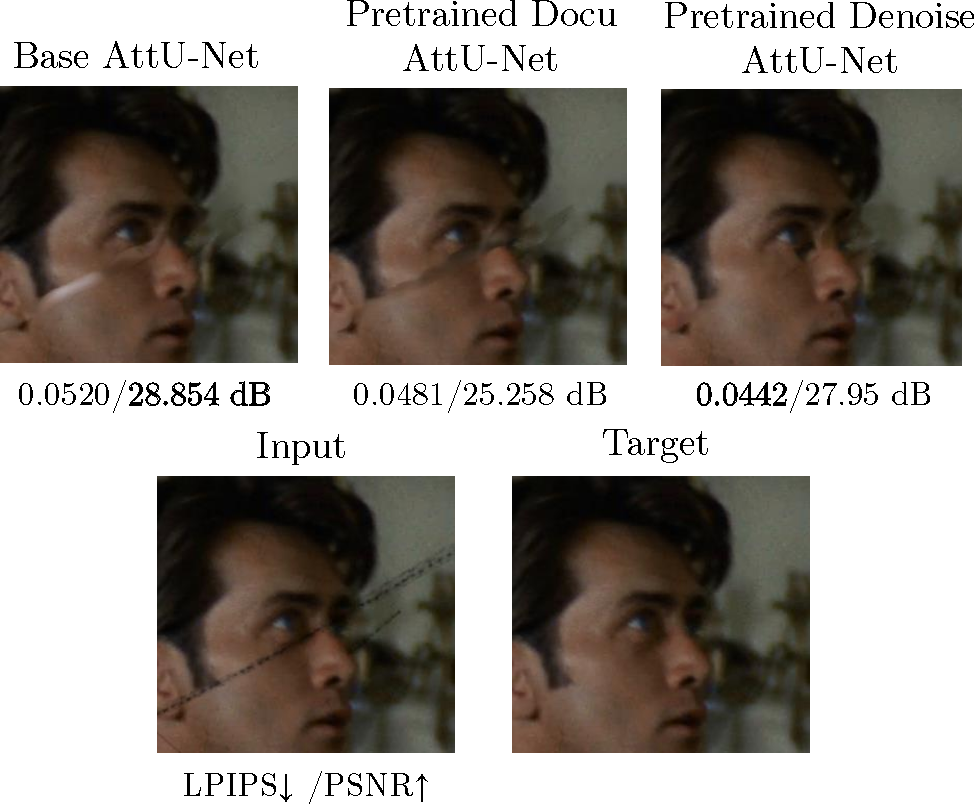
\includegraphics[width=0.8\linewidth]{img/repaint.pdf}
    \caption{\small Comparison of three restorations, using the same three experiments as the AttU-Net experiments used before. It can be observed that now the worst-performing one is the model with the weights initialized using a denoising task. In \textbf{bold} are shown the best performing results in each metric. }
    \label{fig:repaint_comparison}
\end{figure}


\subsubsection{Impact of pretraining and weight initialization}
To assess the role of initialization strategies, experiments were conducted to evaluate three pretraining strategies: no pretraining (random initialization), denoising-only, and domain-specific (Documartica). As shown in Table~1, domain-aligned pretraining consistently improves segmentation performance. The pretrained vanilla U-Net achieves the best overall results, with an average IoU of 0.87 and Dice score of 0.93 across Seen and Unseen splits. Attention U-Net also benefits from Documartica pretraining, outperforming its randomly initialized counterpart.
Denoising pretraining alone yields moderate improvements, particularly in early convergence, suggesting that even generic pretext tasks can help regularize training. However, its final performance remains below that of domain-specific pretraining. These findings emphasize the importance of aligning pretraining objectives and data with the downstream task, particularly in restoration contexts requiring pixel-level precision. As it can be seen in Fig. \ref{fig:segmentation_performance}, a comparasion of the pretraining strategies in the AttU-Net network as well as a mask predicted by the R2AttU-Net, the performance of all three AttU-Net models differ just by a few pixels, even though in this context these pixels are significant, in this case they are not significant enough to determine which one is best. 
\subsubsection{Pixel-Level Sensitivity Analysis}
To better interpret seemingly small differences in segmentation metrics, a pixel-level analysis was conducted comparing predicted damage masks with ground truth annotations. Empirical results indicate that a 0.10 drop in Dice score and a 0.20 drop in IoU correspond to approximately 100 pixels of mismatch per frame. Since artifact regions typically occupy less than 5\% of the total image area, this level of discrepancy is substantial. These results highlight that minor differences in global metrics can reflect significant segmentation failures, especially in fine-grained tasks such as defect localization. Consequently, the performance gap between models like U-Net and R2AttUNet is not only numerically evident but also practically meaningful, with direct implications for restoration accuracy and grain preservation in downstream processing.
\begin{figure*}[t]
    \centering
    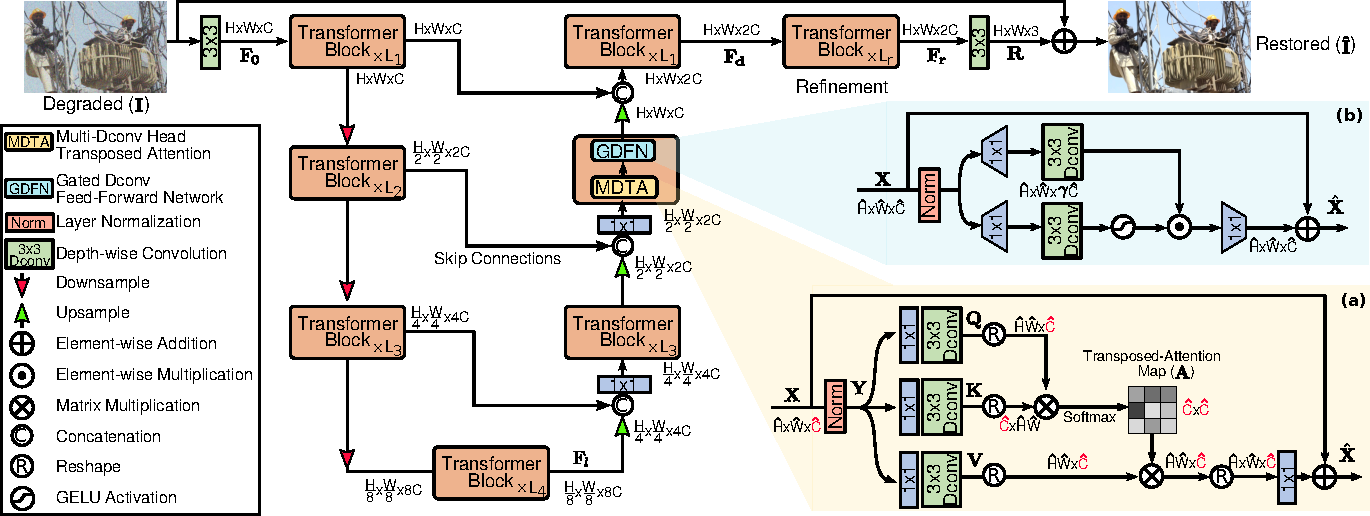
\includegraphics[width= 0.8\textwidth]{img/architecture.pdf}\vspace{-0.6em}
    \caption{Restormer architecture diagram \cite{restormer}. }
    \label{fig:framework}
    \vspace{-1em}
\end{figure*}
\subsubsection{Inpainting Performance}
The inpainting stage, powered by RePaint, operates in a patch-wise manner due to architectural constraints of the pretrained diffusion model. Each high-resolution frame is divided into overlapping $256 \times 256$ tiles, which are inpainted independently and then stitched back together. To reduce computational cost, approximately 30 seconds per tile, diffusion sampling was limited to 25 steps. As a result, processing a single frame (typically composed of 36 tiles) can take over 15 minutes, rendering full-frame inference with higher-quality sampling infeasible for large-scale evaluation. This limitation may partially explain the presence of local artifacts or inconsistencies along patch boundaries, especially on larger artefacts, as it can be seen in Fig. \ref{resultats_repaint}.\\ 
Quantitatively, the inpainting results reported in Table~1 (rightmost columns) are largely consistent with the segmentation performance trends: models producing higher-quality masks (e.g., the pretrained U-Net) yield superior downstream restoration, as reflected in lower LPIPS and higher SSIM and PSNR scores. This alignment confirms the expected pipeline behavior: more accurate segmentation enables more targeted and artifact-aware inpainting. The modular architecture's strength lies precisely in this decoupling, where improvements in one stage directly propagate to the final image quality without retraining the restoration model.


\section{One-Stage Architecture}
In contrast to the modular pipeline, this section explores an end-to-end transformer-based model that directly maps degraded film frames to restored outputs without explicit damage localization. By removing the segmentation stage, this approach relies on the model’s capacity to implicitly identify and correct artifacts, potentially offering a more streamlined restoration workflow.

\subsection{End-to-End Restoration via Implicit Artifact Modeling}
The proposed model is based on Restormer [10], a vision transformer architecture originally designed for high-resolution image restoration tasks such as denoising and deblurring. Unlike the two-stage pipeline that separates defect localization and content synthesis, this model operates in a fully end-to-end fashion. The input is a synthetically degraded film frame, and the output is its restored counterpart.
This formulation treats restoration as a regression problem over all pixels, optimized via an $L_1$ loss. The model receives no auxiliary mask supervision and must implicitly infer both the spatial extent and nature of visual degradations. \\
While this design offers flexibility and generalization, it comes with trade-offs. In the absence of explicit supervision, the model must learn not only how but also where to restore. This increases the risk of modifying visually pristine regions, such as the characteristic grain in analog film, if the learned prior becomes overly aggressive. This behavior contrasts with the two-stage pipeline, where explicit segmentation provides fine-grained control and aligns better with archival restoration principles: intervene only when necessary.

\begin{table*}
\begin{center}
\caption{ \small Restoration performance of the end-to-end Restormer model across various training configurations. The best-performing setup combines the extended dataset and a mask-weighted loss with $\lambda = 0.5$. Arrows indicate whether higher ($\uparrow$) or lower ($\downarrow$) is better. \textbf{Bold} represents the best in that metric, and \underline{underlined} the second best. The final row represents the combination of the best performing experiments: Trained with the big dataset, a weighted L1 loss with $\lambda=0.5$, and pretrained.}
\label{table:restormer_results}
\vspace{-2mm}
\setlength{\tabcolsep}{10pt}
\scalebox{0.75}{
\begin{tabular}{l ccc|ccc || ccc}
\toprule[0.15em]
\textbf{Method} 
& \multicolumn{3}{c|}{\textbf{Seen}} 
& \multicolumn{3}{c||}{\textbf{Not Seen}} 
& \multicolumn{3}{c}{\textbf{Average}} \\
& LPIPS $\downarrow$ & PSNR $\uparrow$ & SSIM $\uparrow$ 
& LPIPS $\downarrow$ & PSNR $\uparrow$ & SSIM $\uparrow$ 
& LPIPS $\downarrow$ & PSNR $\uparrow$ & SSIM $\uparrow$ \\
\midrule[0.15em]
Baseline (small dataset) & 0.0169 & 30.72 & 0.9957 & 0.0236 & 31.94 & 0.9947 & 0.0203 & 31.33 & 0.9952 \\
Extended Dataset Only  & \underline{0.0042} & 33.67 & 0.9979 & \textbf{0.0036} &  \underline{35.50} & \textbf{0.9982} & \textbf{0.0039} & 34.59 & \textbf{0.9981} \\
Large Patches Only & 0.0158 & 28.32 & 0.9947 & 0.0186 & 29.61 & 0.9951 & 0.0172 & 28.97 & 0.9949 \\
Deraining finetunning & 0.0043 & 33.97 & \underline{0.9981} & \underline{0.0075} & 34.78 & 0.9965 & \underline{0.0059} & 34.38 & \underline{0.9973} \\
Masked Loss ($\lambda = 0$) & 0.0610 & 30.88 & 0.9749 & 0.0482 & 32.53 & 0.9762 & 0.0546 & 31.70 & 0.9756 \\
Masked Loss ($\lambda = 0.01$) & 0.0188 & 32.29 & 0.9908 & 0.0157 & 34.01 & 0.9917 & 0.0173 & 33.15 & 0.9913 \\
Masked Loss ($\lambda = 0.25$) & 0.0066 & 34.17 & 0.9976 & 0.0158 & 34.37 & 0.9938 & 0.0112 & 34.27 & 0.9957 \\
Masked Loss ($\lambda = 0.50$) & \textbf{0.0031} & \textbf{35.87} & 0.9984 & 0.0153 & \textbf{36.00} & \underline{0.9876} & 0.0092 & \textbf{35.94} & 0.9930 \\
Masked Loss ($\lambda = 0.75$) & 0.0044 & \underline{34.51} & \textbf{0.9980} & 0.0144 & 34.80 & 0.9907 & 0.0094 & \underline{34.66} & 0.9944 \\
\midrule[0.15em]
\textbf{Final Model} 
& \textbf{0.0023} & \textbf{36.90} & \textbf{0.9985} 
& \textbf{0.0032} & \textbf{35.33} & \textbf{0.9982} 
& \textbf{0.0028} & \textbf{36.12} & \textbf{0.9983} \\
\bottomrule[0.1em]
\end{tabular}}
\end{center}
\vspace{-1.5em}
\end{table*}
\subsection{Restormer Architecture and Vision Transformer Principles}
Restormer \cite{restormer} is selected in this work for its ability to model long-range dependencies via attention mechanisms while preserving spatial resolution, an essential property for film restoration tasks involving spatially extended degradations. Unlike convolution-based architectures with fixed receptive fields, Restormer dynamically aggregates contextual information through self-attention, making it particularly effective for detecting and restoring artifacts such as scratches or stains that span non-local image regions.
\subsection{Experimental Setup}
To evaluate the end-to-end restoration model, a sequence of controlled experiments is conducted using synthetically generated degraded-clean image pairs. The objective is to assess the model's capacity to reconstruct corrupted content while preserving perceptual fidelity, particularly the fine-grain and texture characteristics of analog film. The experimental sequence begins with a baseline configuration and iteratively introduces modifications to the data volume, architectural parameters, and loss function. Each variant is designed to address limitations identified in preceding configurations.
\subsubsection{Baseline Training Configuration}
The initial model is trained using the synthetic dataset described in Section~\ref{sec:dataset}, containing approximately 1,300 image pairs. Restoration is formulated as a pixel-wise regression problem, optimized using the standard $\ell_1$ loss:
\begin{equation*}
\mathcal{L}_{L1} = \dfrac{1}{N} \sum_{i=1}^{N} \left| \hat{I}_i - I_i \right|
\end{equation*}
Training is conducted for 100{,}000 iterations with a batch size of 4 and an initial learning rate of $4 \times 10^{-3}$. All other settings follow the default configuration of the Restormer architecture.
\subsubsection{Identifying Limitations and Scaling Data}
Despite achieving visually coherent restorations on training-domain samples, the baseline model exhibits limited generalization to unseen visual styles and degradation patterns. This is attributed to the relatively small and stylistically homogeneous dataset used for training. To address this, a new synthetic dataset is constructed containing approximately 5,000 image pairs. This expanded dataset introduces greater diversity in film stocks, textures, and artifact types, while maintaining the same artifact simulation pipeline as before. The aim is to provide broader visual coverage and stronger inductive bias during training.
\subsubsection{Evaluating Patch Size Effects}
The original Restormer implementation~\cite{restormer} was designed for image resolutions of 256×256 pixels, using small patch sizes during training. Since the film scans in this work have approximately twice the resolution, it is hypothesized that the default patch configuration may limit the model's receptive field and its ability to handle large-scale degradations. To investigate this, an additional model is trained using larger input patches, approximately double the default size, while keeping the total number of training iterations and optimization parameters unchanged. This experiment is intended to evaluate whether increasing spatial context during training improves the consistency of restored outputs.

\subsubsection{Domain-Specific Finetuning}

To assess the adaptability of pretrained transformer-based models to the film restoration task, a finetuning experiment was conducted using the deraining model provided by the original Restormer paper~\cite{restormer}. This model, originally trained to remove synthetic rain artifacts from natural images, was repurposed by further training on the synthetic film degradation dataset introduced in this work. \\
Finetuning was performed for several epochs using the same $\ell_1$ loss (sum-reduced) and learning rate schedule as in the baseline setup. The goal of this experiment is to evaluate whether a pretrained model, initially optimized for a visually distinct task, can transfer effectively to the domain of analog film restoration. This setup also serves as a practical alternative to full training in scenarios with limited compute or data availability.
\subsubsection{Enhancing Focus via Loss Reweighting}
An initial observation during training was that the standard $\ell_1$ loss converged slowly, with low-magnitude gradients. This was due to the majority of pixels being uncorrupted, causing the loss to be dominated by regions requiring no restoration. \\\ To address this, the loss reduction was changed from mean to sum, allowing the loss magnitude, and thus the gradient strength, to scale with the number of corrupted pixels. This led to slightly more stable convergence and improved restoration in affected areas. \\ Building on this, a mask-weighted $\ell_1$ loss was introduced to explicitly reweight contributions from damaged and undamaged regions. Corrupted pixels received full weight, while clean ones were downweighted using a factor $\lambda \in {0, 0.1, 0.25, 0.5, 0.75}$:
\begin{equation*}
\mathcal{L}_{\text{weighted}} = \sum_{i=1}^N \left[ M_i \cdot |\hat{I}_i - I_i| + \lambda (1 - M_i) \cdot |\hat{I}_i - I_i| \right]
\end{equation*}
where $M_i$ is a binary mask indicating artifact-affected pixels, computed by thresholding the absolute difference between degraded and clean frames. The sum reduction is retained in this formulation, as preliminary comparisons showed that it yielded better results than the mean-reduced counterpart across multiple $\lambda$ values. This reweighting scheme allows the model to prioritize learning on challenging, artifact-heavy regions while maintaining global consistency.
\subsubsection{Evaluation Metrics}
Restoration quality was evaluated using the same metrics defined in Section \ref{experimental_setup_metrics} for consistency and ability to compare. Quantitative assessments included PSNR, SSIM, and LPIPS. 

\subsection{Results and Discussion}

This section presents the results of the one-stage restoration experiments introduced previously. Table~\ref{table:restormer_results} reports the quantitative performance of each model on both Seen and Unseen evaluation splits.

\subsubsection{Baseline Performance}

The baseline model, trained on the original synthetic dataset with standard $\ell_1$ loss and mean reduction, achieved strong perceptual quality on Seen data (LPIPS = 0.0169, SSIM = 0.9957). However, performance on Unseen domains, films, and styles not present in the training set was less consistent. This gap highlighted limitations in generalization and motivated further exploration.

\subsubsection{Effect of Data Scaling}

Training with the expanded dataset yielded the most immediate improvement. The model trained on the extended 5k-pair dataset significantly outperformed the baseline across all metrics and both evaluation splits. LPIPS dropped to 0.0039, and PSNR increased by over 3 dB on average. These results confirm that increasing stylistic diversity and artifact variation in training data has a substantial impact on generalization.
\begin{figure*}[t]
    \centering
    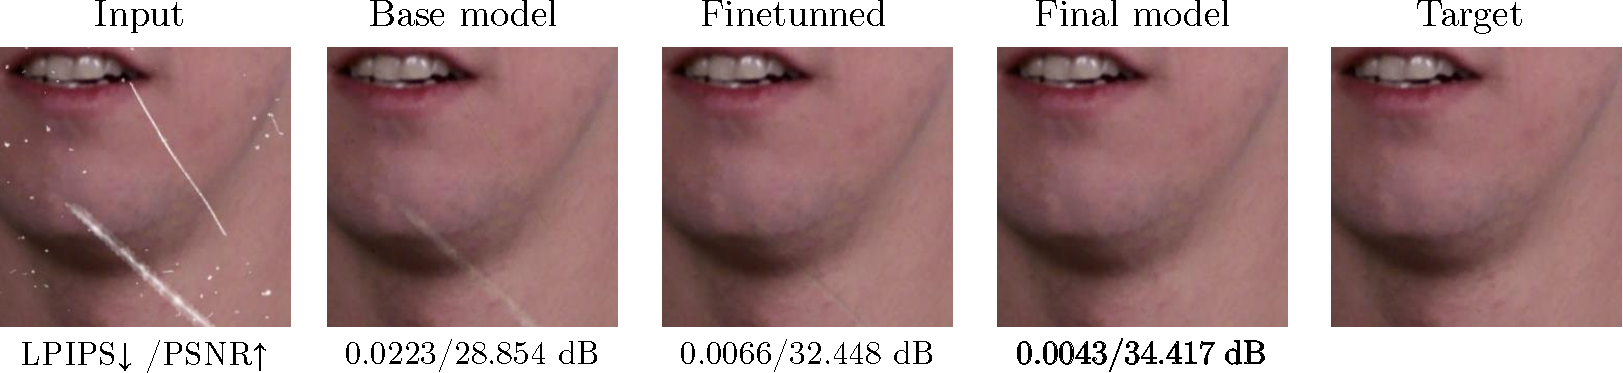
\includegraphics[width= \textwidth]{img/comparason_restormer.pdf}\vspace{-0.6em}
    \caption{\small Results across three selected restormer tests, the baseline model, the finetuned model from the existing deraining weights, and the final model containing all the better-performing experiments. As can be seen, there is a significant improvement from the baseline to the final model, both quantitatively and qualitatively.}
    \label{fig:comparason_restormer}
    \vspace{-1em}
\end{figure*}
\subsubsection{Effect of Larger Patch Sizes}

Contrary to expectations, increasing the patch size without curriculum learning led to degraded performance. The fixed large-patch model underperformed on both seen and Unseen data, with LPIPS increasing and PSNR decreasing compared to the baseline. This suggests that increasing the receptive field alone is insufficient and may compromise local fidelity, particularly critical for preserving film grain and sharp details.
\subsubsection{Effect of Domain-Specific Finetuning}

Finetuning the original Restormer deraining model on the synthetic film restoration dataset yielded measurable improvements over training from scratch. On the Unseen evaluation split, performance improved across all metrics, indicating that prior exposure to a related low-level restoration task, despite differing visual artifacts, can accelerate adaptation and improve generalization. However, these gains remained modest compared to models trained from the ground up on the full extended dataset. This suggests that while task-transfer finetuning is beneficial, full retraining on domain-specific data remains more effective when resources permit.
\subsubsection{Loss Reweighting: Precision on Damaged Regions}

Changing the $\ell_1$ loss reduction from mean to sum resulted in modest improvements, confirming that small loss magnitudes were indeed limiting the gradient signal. Building on this, the use of a mask-weighted loss with $\lambda = 0.5$ led to substantial improvements in restoration quality. This variant achieved an average PSNR of 35.94 and the lowest LPIPS score (0.0092) among all tested models. These results validate the importance of prioritizing corrupted regions during training, while still maintaining some supervision over clean areas.
\begin{table*}
\begin{center}
\caption{ \small Comparison of final models across seen and unseen data. The One-Stage Final Model clearly outperforms the two-stage pretrained U-Net baselines both in restoration quality and inference speed. In \textbf{bold} the best result in each metric, and underlined the second best.}
\label{table:final_model_results}
\vspace{-2mm}
\setlength{\tabcolsep}{10pt}
\resizebox{\textwidth}{!}{
\begin{tabular}{l ccc|ccc || ccc|c}
\toprule[0.15em]
\textbf{Method} 
& \multicolumn{3}{c|}{\textbf{Not Seen}} 
& \multicolumn{3}{c||}{\textbf{Seen}} 
& \multicolumn{3}{c|}{\textbf{Average}} 
& Time/frame (s) $\downarrow$ \\
& LPIPS $\downarrow$ & PSNR $\uparrow$ & SSIM $\uparrow$ 
& LPIPS $\downarrow$ & PSNR $\uparrow$ & SSIM $\uparrow$ 
& LPIPS $\downarrow$ & PSNR $\uparrow$ & SSIM $\uparrow$ 
& \\
\midrule[0.15em]
Two-Stage (Pretrained AttU-Net) & 0.0387 & \underline{26.46} & 0.9765 & \underline{0.0399} & \underline{25.90} & \underline{0.9754} & \underline{0.0393} & \underline{26.18} & 0.9760 & 432.00 \\
Two-Stage (Pretrained U-Net) & \underline{0.0382} & 26.01 & \underline{0.9766} & 0.0409 & 25.37 & 0.9754 & 0.0396 & 25.69 & \underline{0.9760} & \underline{396.00} \\
One-Stage (Final Restormer model) & \textbf{0.0023} & \textbf{36.90} & \textbf{0.9985} & \textbf{0.0032} & \textbf{35.33} & \textbf{0.9982} & \textbf{0.0027} & \textbf{36.12} & \textbf{0.9984} & \textbf{1.32} \\
\bottomrule[0.1em]
\end{tabular}}
\end{center}
\vspace{-1.5em}
\end{table*}
\subsubsection{Final Model}

The best results were obtained by combining the two most effective improvements: the extended dataset and the mask-weighted loss with $\lambda = 0.5$. This final model demonstrated the strongest average performance across all metrics, including Seen and Unseen subsets. It is used as the representative end-to-end model for the comparative evaluation in the next Section.

\section{Global Results and Discussion}
 This section presents a comparative analysis of the two most effective models, one from each architectural family, based on quantitative evaluation metrics and a qualitative test using a real-world film scan. The goal is to assess not only which model performs better under synthetic conditions, but also which model does it faster and more efficiently. Qualitative results comparison can be seen in Appendix B.
\subsection{Quantitative Comparison on Synthetic Test Set}
Table~\ref{table:final_model_results} compares the best-performing models from both the two-stage and one-stage pipelines. The final Restormer-based one-stage model clearly outperforms the pretrained U-Net and AttU-Net baselines across all quantitative metrics. \\
On unseen data, the Restormer achieves a significantly lower LPIPS of 0.0023, alongside a PSNR of 36.90 dB and an SSIM of 0.9985. In contrast, the two-stage models remain in the 0.038–0.039 LPIPS range and below 26.5 dB PSNR. On seen data, the gap remains consistent: the one-stage model improves PSNR by nearly 10 dB and raises SSIM from around 0.975 to 0.9982. \\
In addition to superior restoration quality, the Restormer model offers a dramatic reduction in inference time, requiring only 1.32 seconds per frame, compared to 396 seconds for the U-Net and 432 seconds for the AttU-Net. This improvement of over 300× in speed further reinforces the practicality of the one-stage design. 

These results confirm that the final Restormer model not only sets a new benchmark in restoration quality but also delivers the computational efficiency needed for scalable deployment. 
\subsection{Qualitative evaluation on real scans}
Beyond synthetic benchmarks, the true value of a restoration model lies in its performance on real degraded film scans. A qualitative test was conducted on a high-resolution 35mm scan featuring typical artifacts, scratches, dust, and dirt, unseen during training. \\
Both models were evaluated: the two-stage approach delivered more consistent, artifact-aware results, with its segmentation network enabling selective inpainting that preserved undamaged areas and natural grain. Restormer, while visually effective in parts, often failed to correct defects and introduced mild oversharpening. \\
This gap likely reflects differences in generalization. Despite fewer training iterations, the two-stage model better handled real-world degradation, whereas Restormer, trained longer, struggled with unseen artifacts, suggesting transformer-based models may require broader data to generalize well. \\
While these results point to the robustness of the modular pipeline under limited data, broader evaluation on diverse real scans remains future work.
\section{Limitations and Future Work}
While this work offers valuable insight into the strengths of modular versus end-to-end architectures for analog film restoration, several limitations must be noted. \\ The one-stage solution, despite achieving top scores on synthetic benchmarks, struggled with real scanned footage, highlighting limited data efficiency and suggesting that transformer-based models may require broader and longer training to generalize. Only one extended training setup was explored due to time constraints. The qualitative evaluation was also limited to a single real scan. Although results favored the one-stage model, further testing across varied sources is needed to validate its generalizability. Moreover, evaluating real scans objectively remains challenging without ground truth. \\ One promising future direction is incorporating temporal context into the restoration process. Artifacts like dust and scratches are often transient across frames, while scene content is temporally coherent. Exploiting this could improve both defect detection and restoration quality.\\ Overall, this work lays the groundwork for comparative evaluation, and future work should expand real-world testing, scale training strategies, and explore temporal modeling for improved restoration of analog film.
\section{Conclusions}
This project compared two deep restoration pipelines for scanned 35mm film: a modular two-stage system and an end-to-end transformer-based model. Both were designed to remove artifacts such as dust and scratches while preserving the original film grain, a key restoration goal. \\
The two-stage approach, combining damage segmentation with mask-guided inpainting, proved easier to set up and more interpretable. It offered fine-grained control, allowing restorations that altered only damaged areas. This led to minimal interference with grain, especially on real-world footage, where it consistently avoided over-restoration. \\
In contrast, the end-to-end Restormer model unified restoration into a single network. Though harder to train, it produced faster inference and performed better on synthetic benchmarks. However, it sometimes modified clean regions, including grain, due to the lack of explicit damage supervision. \\
Both methods are feasible and effective, with distinct trade-offs. The two-stage design excels in precision and archival alignment; the end-to-end model is better suited for scalable deployment. Future work could explore hybrid designs and temporal consistency to enhance both quality and generalization.

\section{Acknowledgements}
I would like to thank Dr. Ramon Baldrich i Caselles for granting me access to the Computer Vision Center and for his continuous support, guidance, and knowledge throughout this project. I would also like to thank all the CVC interns who were present for their help and encouragement during the development of this work.
\begingroup
\small  % or \footnotesize, \scriptsize, etc.
\renewcommand{\refname}{References}
\bibliography{references}
\bibliographystyle{plain}
\endgroup
\onecolumn
\appendix
\section{Dataset examples}

\begin{figure}[h]
    \centering
    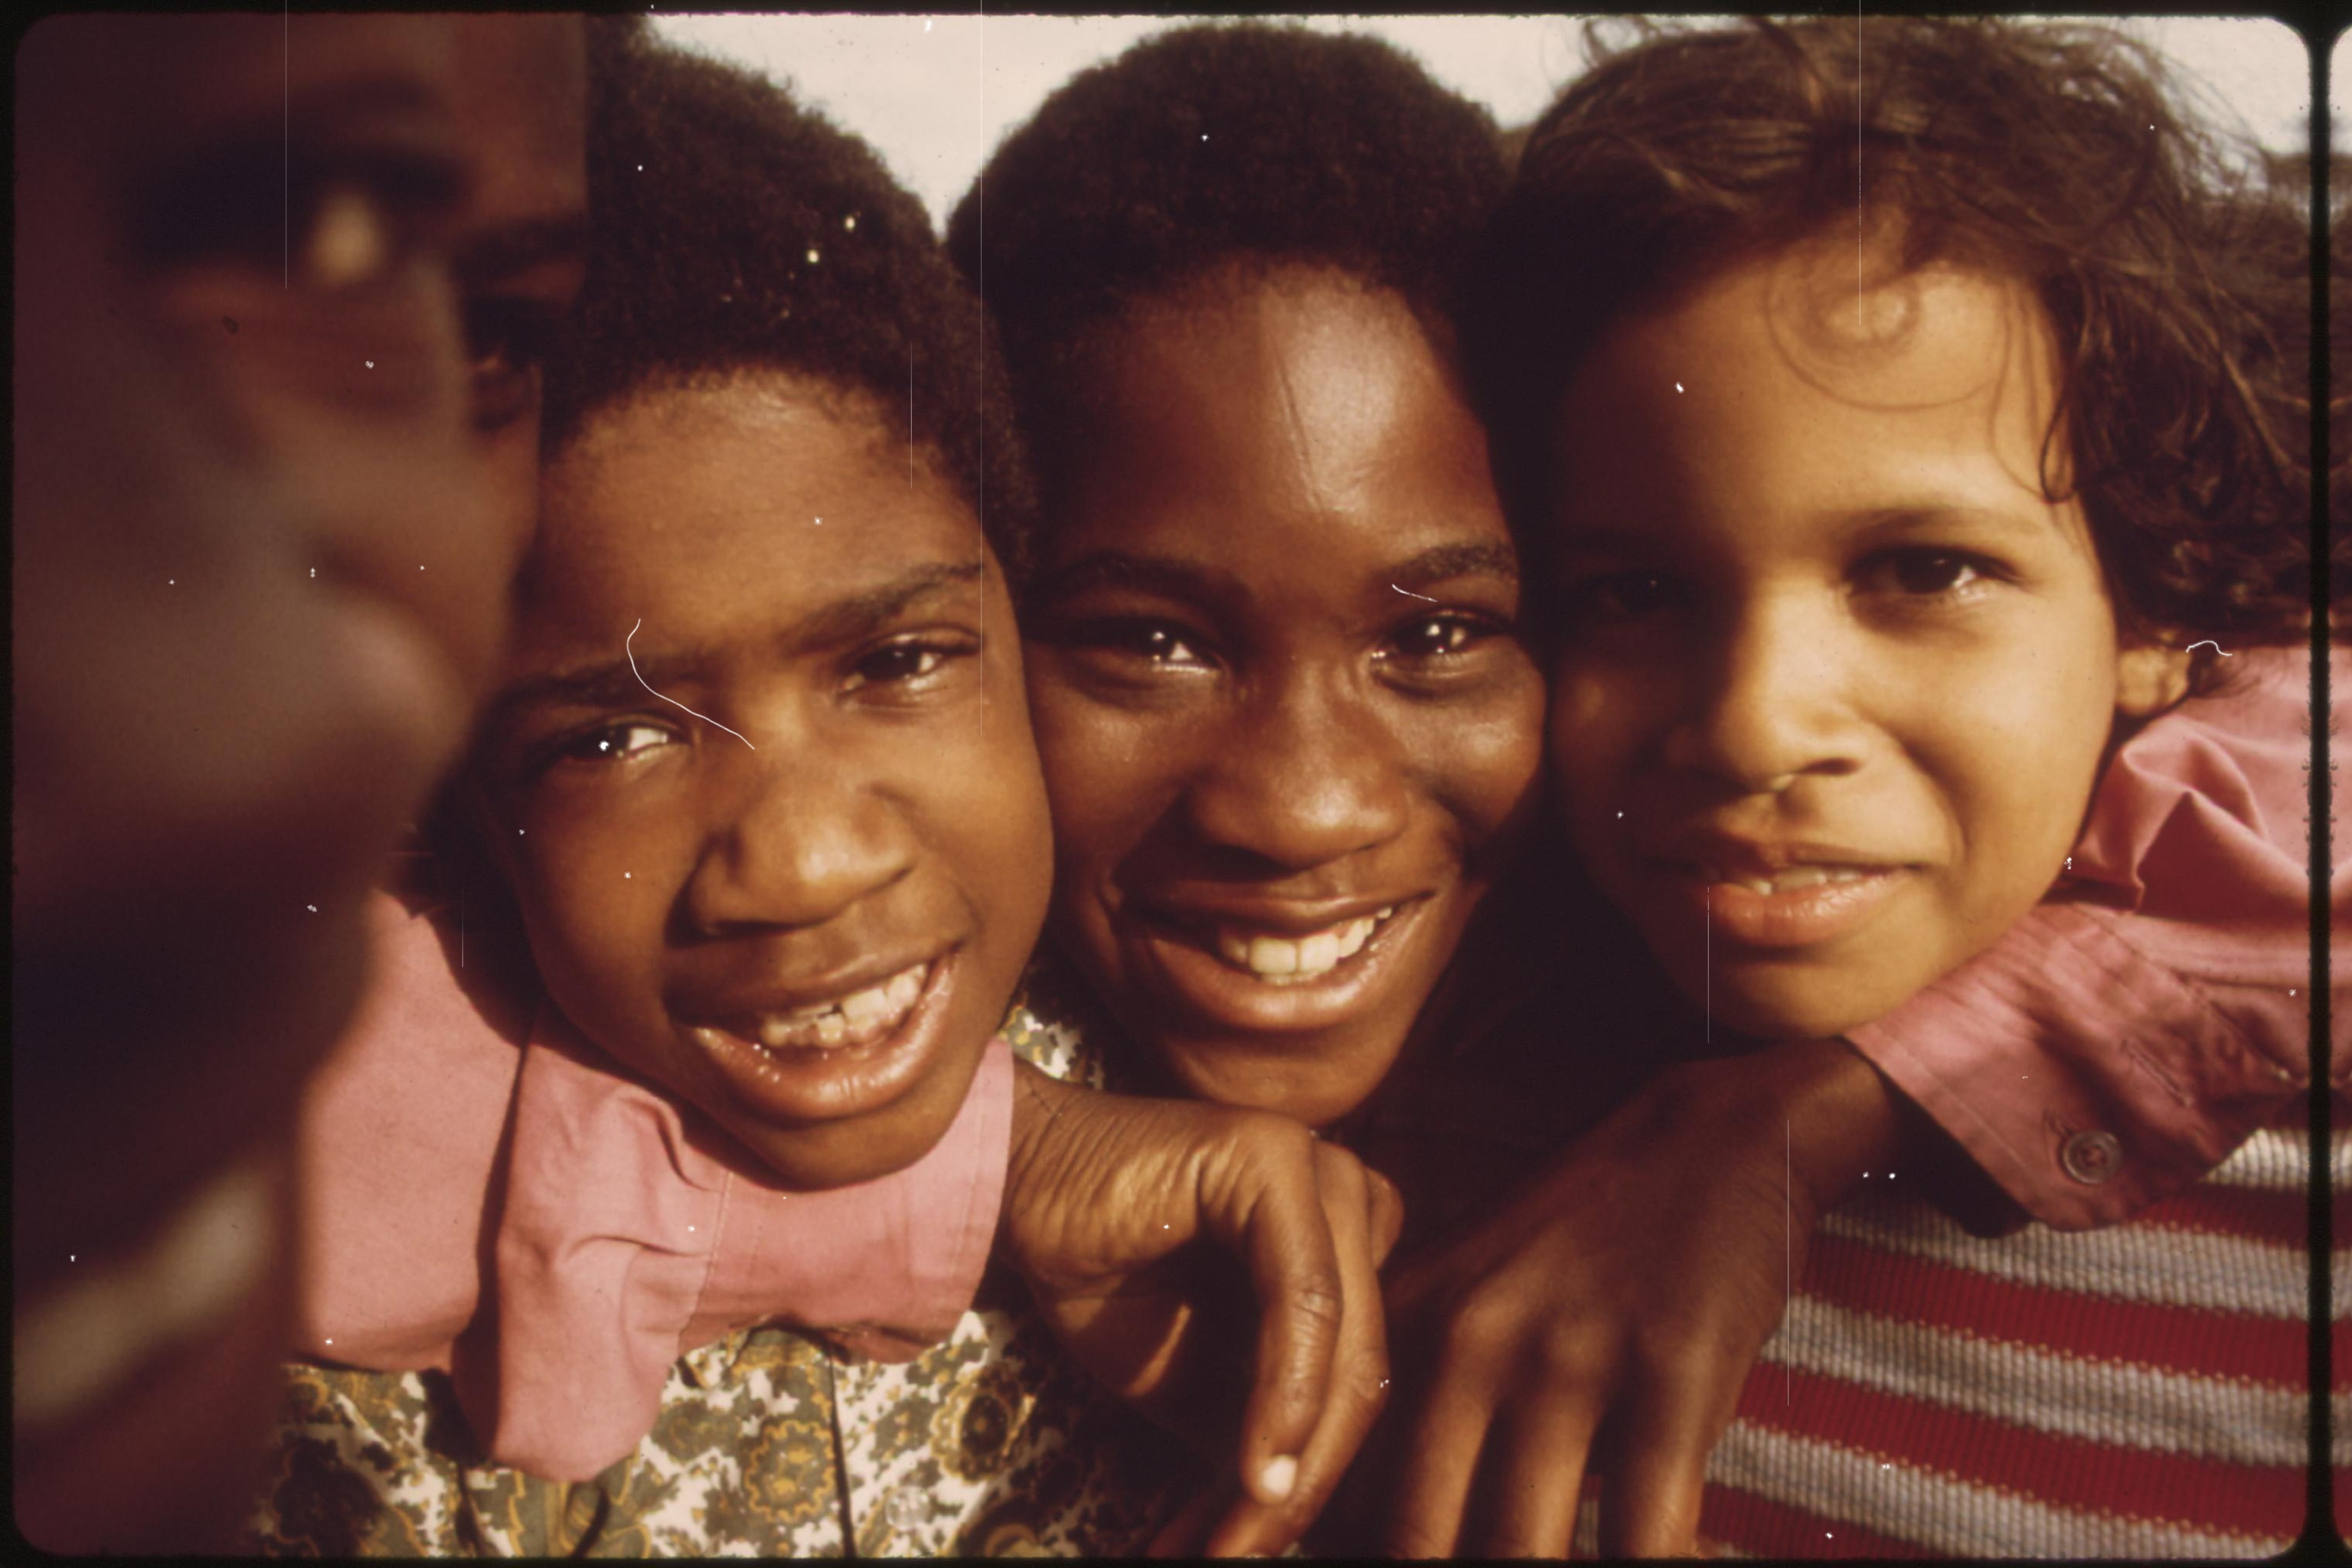
\includegraphics[width=0.6\linewidth]{img/docu.jpg}
    \caption{Example image from the Documartica dataset.}
    \label{fig:anex1}
\end{figure}
\begin{figure}[h]
    \centering
    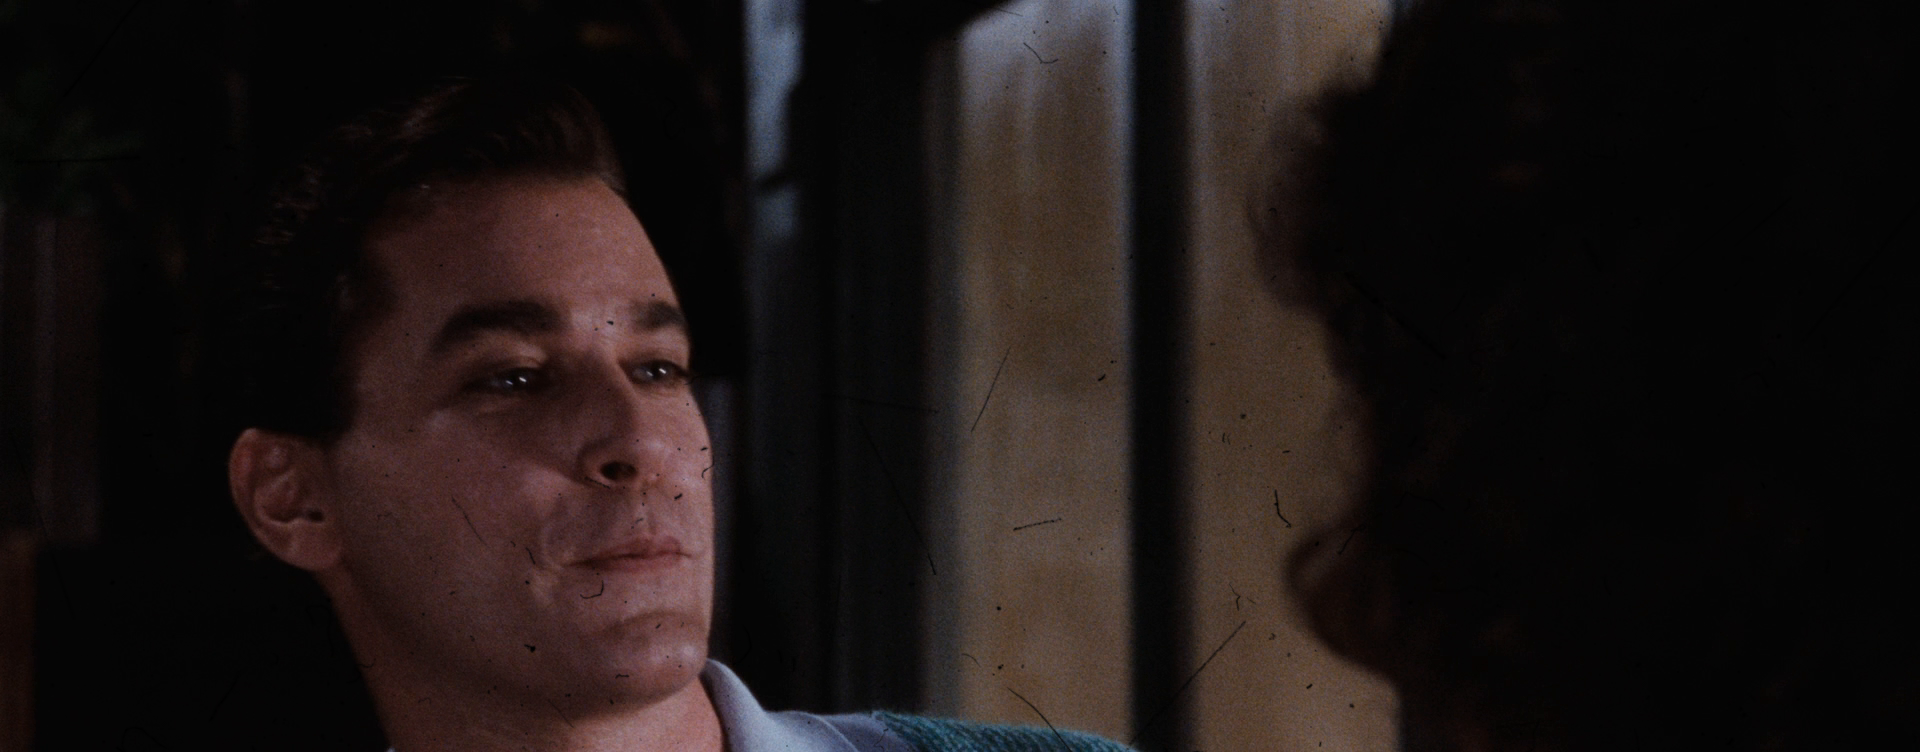
\includegraphics[width=0.7\linewidth]{img/goodfellas_frame_0113.png}
    \caption{Example dirty frame from the synthetic dataset.}
    \label{fig:anex2}
\end{figure}
\begin{figure}[h]
    \centering
    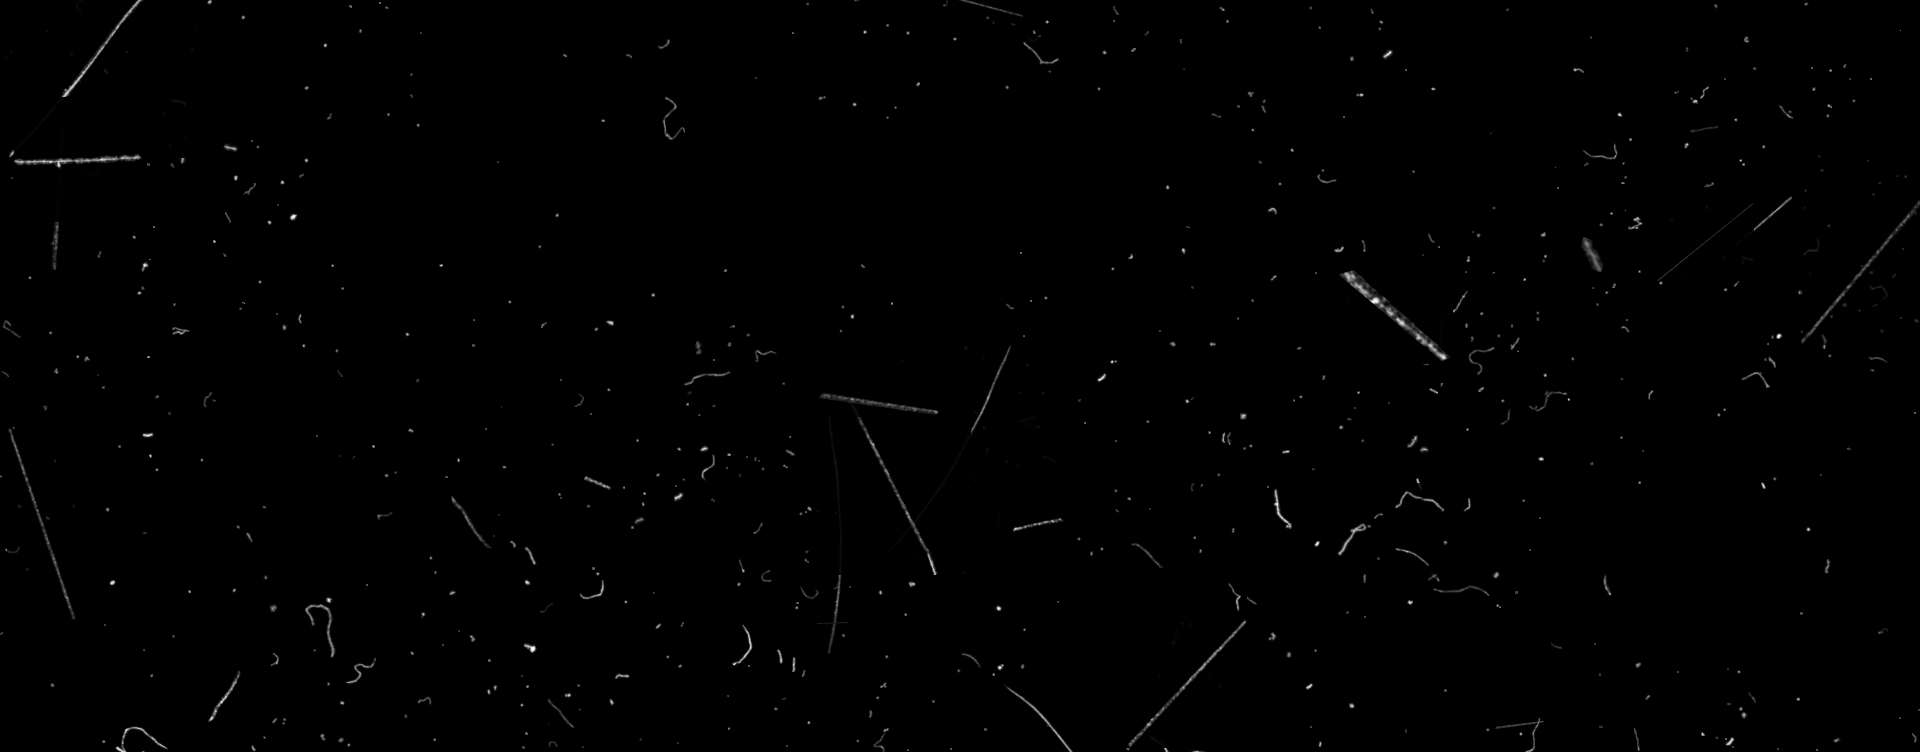
\includegraphics[width=0.7\linewidth]{img/inverse_mask.png}
    \caption{Example mask label from the synthetic dataset.}
    \label{fig:anex3}
\end{figure}
\newpage
\section{Additional Results}

\begin{figure}[h]
    \centering
    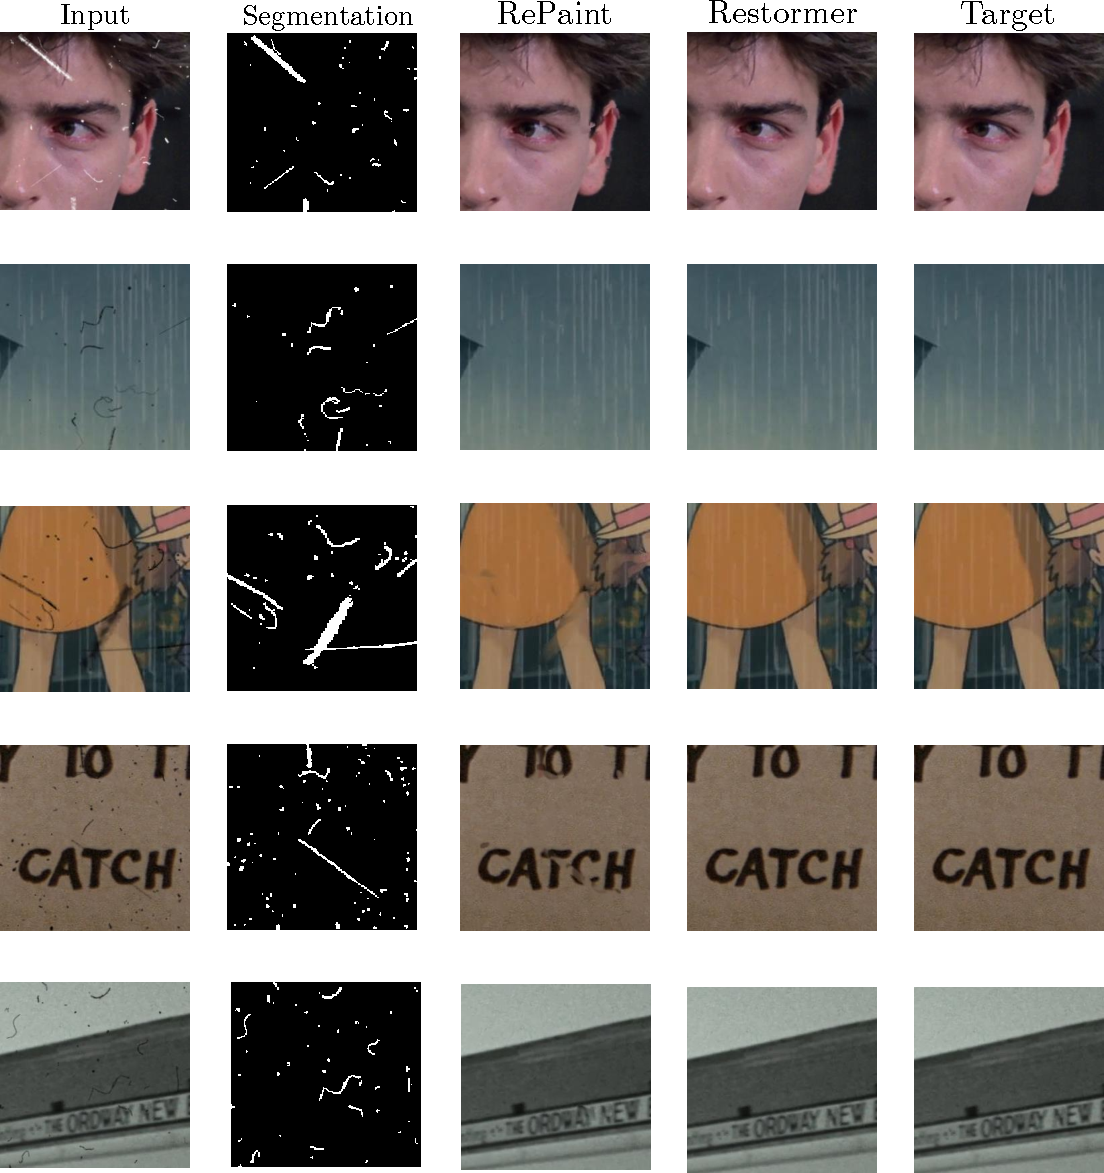
\includegraphics[width=0.8\linewidth]{img/AnnexA.pdf}
    \caption{Additional qualitative comparison of the models' performance. For the two-stage section, the pretrained U-Net was used, and for the Restormer, the final model training was used (trained with the weighted L1 loss with $\lambda = 0.5$, finetunning the original deraining model with the big dataset). Qualitatively, it can be determined that the one-stage model is not only faster, but also the better-performing one. }
    \label{fig:anex5}
\end{figure}
\end{document}
